\section{The Big Picture}
\begin{frame}{The Big Picture}{\linux \& Co.}
 \begin{block}{einerseits}
  \begin{itemize}
   \item besteht \linux aus nur ein paar Komponenten
   \item ist \linux relativ modern
  \end{itemize}
 \end{block}
 \begin{block}{andrerseits}
  \begin{itemize}
   \item ist \linux sehr komplex
   \item ist \linux klassisch hergestellt
   \begin{itemize}
    \item mit �ber 30-j�hrigen Konzepten
   \end{itemize}
  \end{itemize}
 \end{block}
\end{frame}

\begin{frame}{Die Komponenten}{layers}
\begin{center}
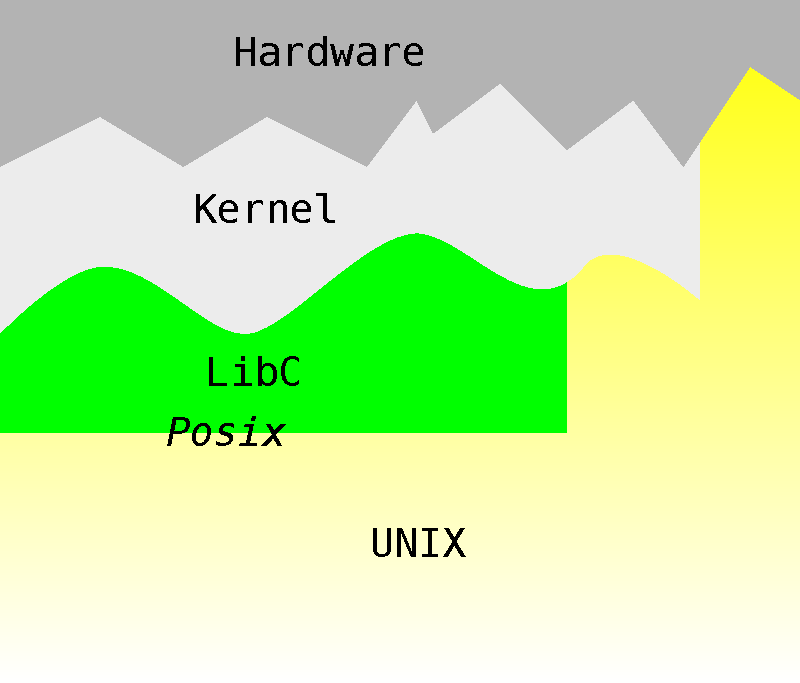
\includegraphics[width=9cm]{layers.pdf}
\end{center}
\end{frame}

\begin{frame}{Die Komponenten}
 \begin{description}
  \item[HW] heterogen:
  \begin{itemize}
   \item Architekturen \arm, {\em Intel}
   \item Peripherie 
  \end{itemize}
  \item[Kernel] das eigentliche \linux
  \begin{itemize}
   \item Sammlung von {\em drivern}
   \item Scheduling
   \item Verwaltung der Resourcen
  \end{itemize}
  \item[LibC] die POSIX Norm
  \begin{itemize}
   \item {\tiny\url{http://pubs.opengroup.org/onlinepubs/9699919799/}}
  \end{itemize}
  \item[\unix] der Rest:
  \begin{itemize}
   \item alles ist ein File
  \end{itemize}
 \end{description}
\end{frame}

\begin{frame}{Die Komplexit�t}
 \begin{block}{Zwei Beispiele}
 \begin{itemize}
   \item die {\em include} Relationen im {\em kernel}
   \item die Verzeichnisstruktur einer \unix Workstation
 \end{itemize}
 \end{block}
\end{frame}

\begin{frame}{Include Relationen}{nur im \kernel}
\vspace{-3.5mm}
\begin{center}
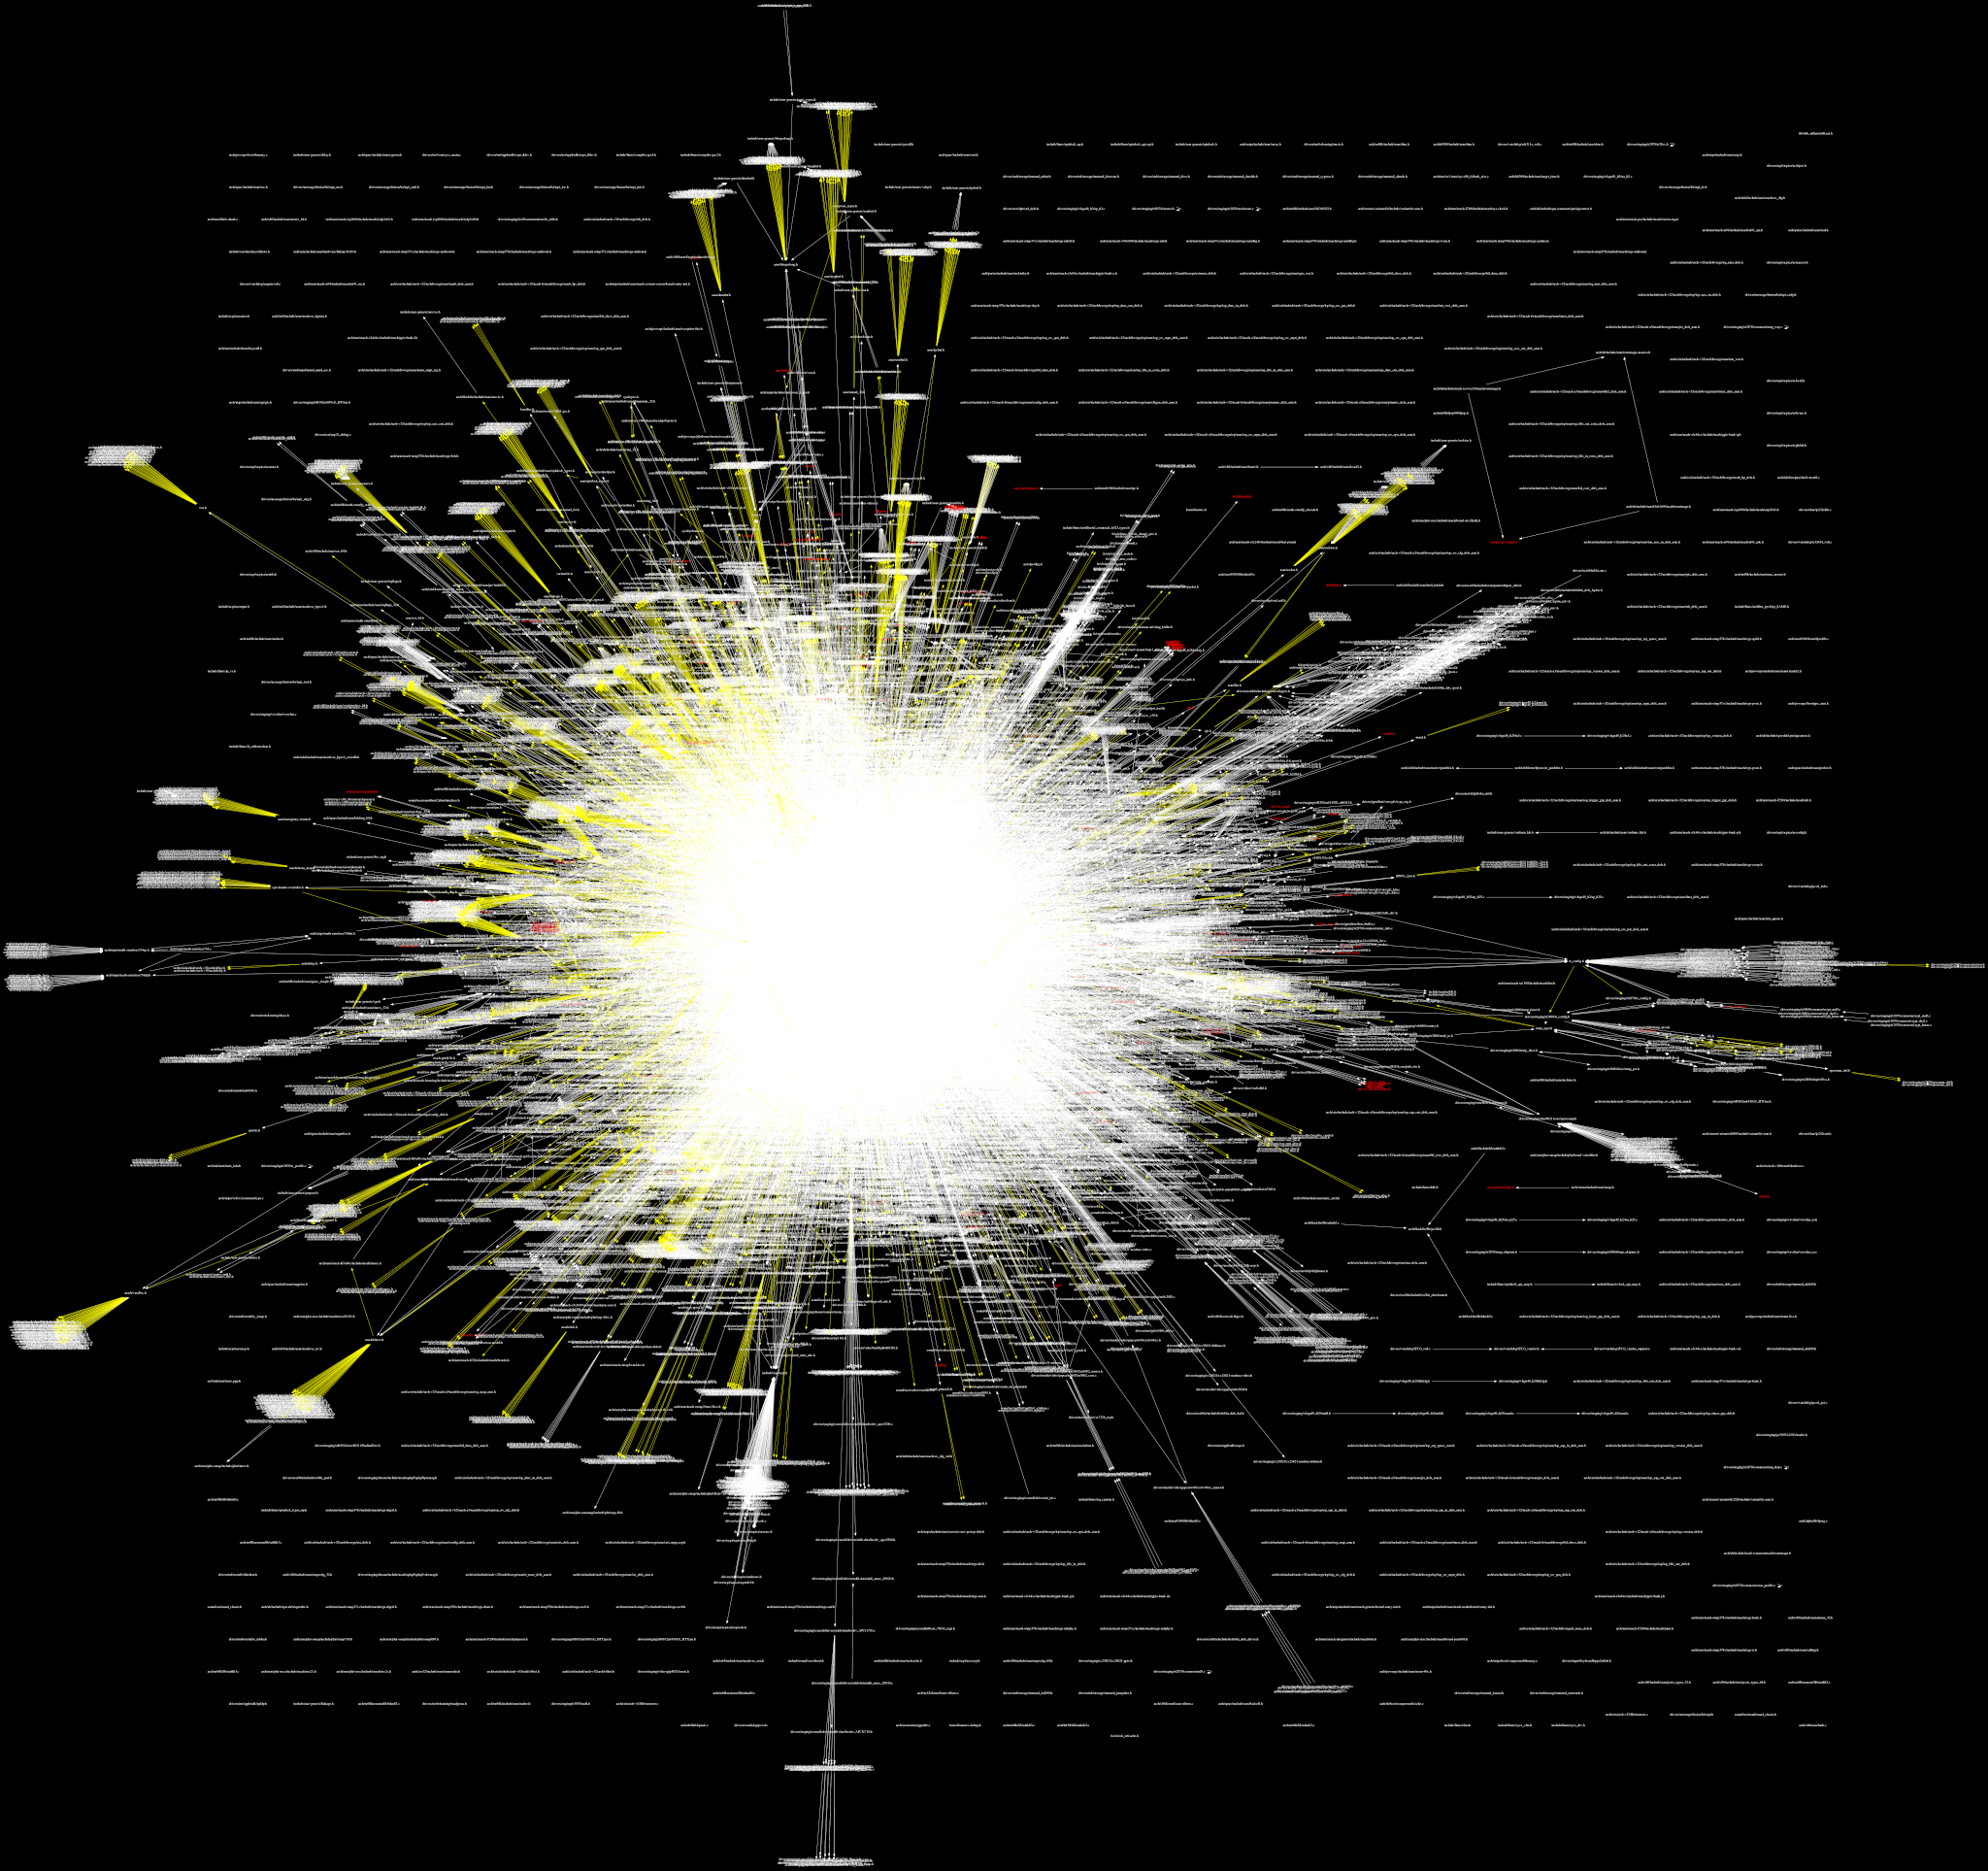
\includegraphics[height=8cm]{include-small.png}
\end{center}
\end{frame}

\begin{frame}{Verzeichnisstruktur}{einer Workstation}
\vspace{-5mm}
\begin{center}
 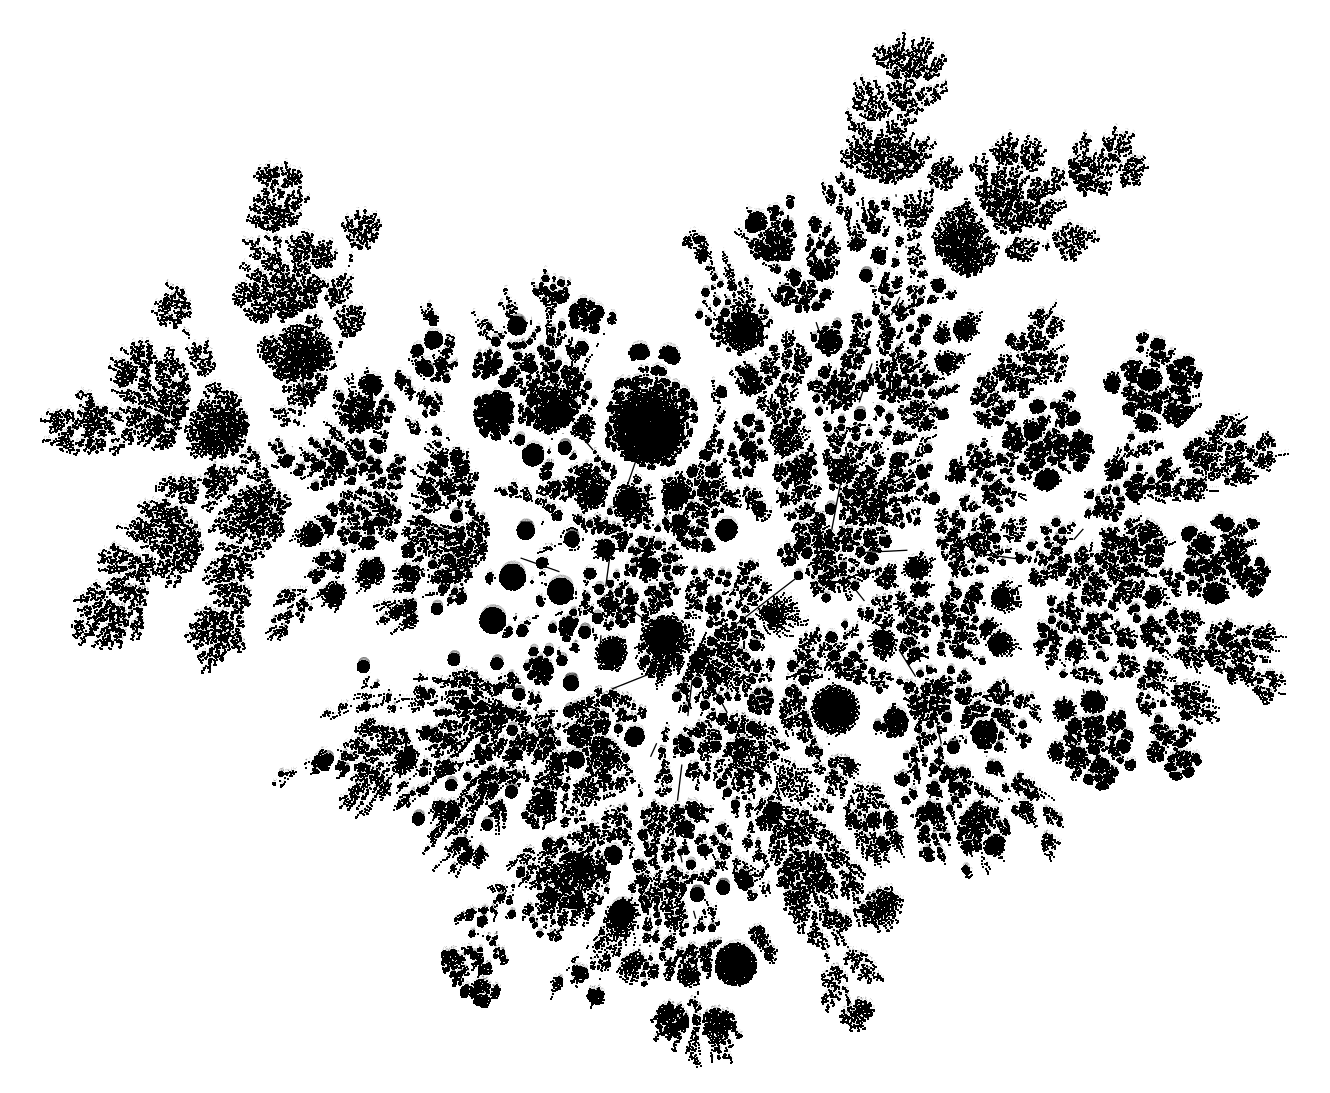
\includegraphics[height=7cm]{directories.png}
\end{center}
\end{frame}

\begin{frame}{Die Herstellung}{die klassischen Methoden}
 \begin{description}[\cod{make}]
  \item[\C] die dominante Programmiersprache
  \item[\cod{make}] Steuerung der Herstellung
 \end{description}
  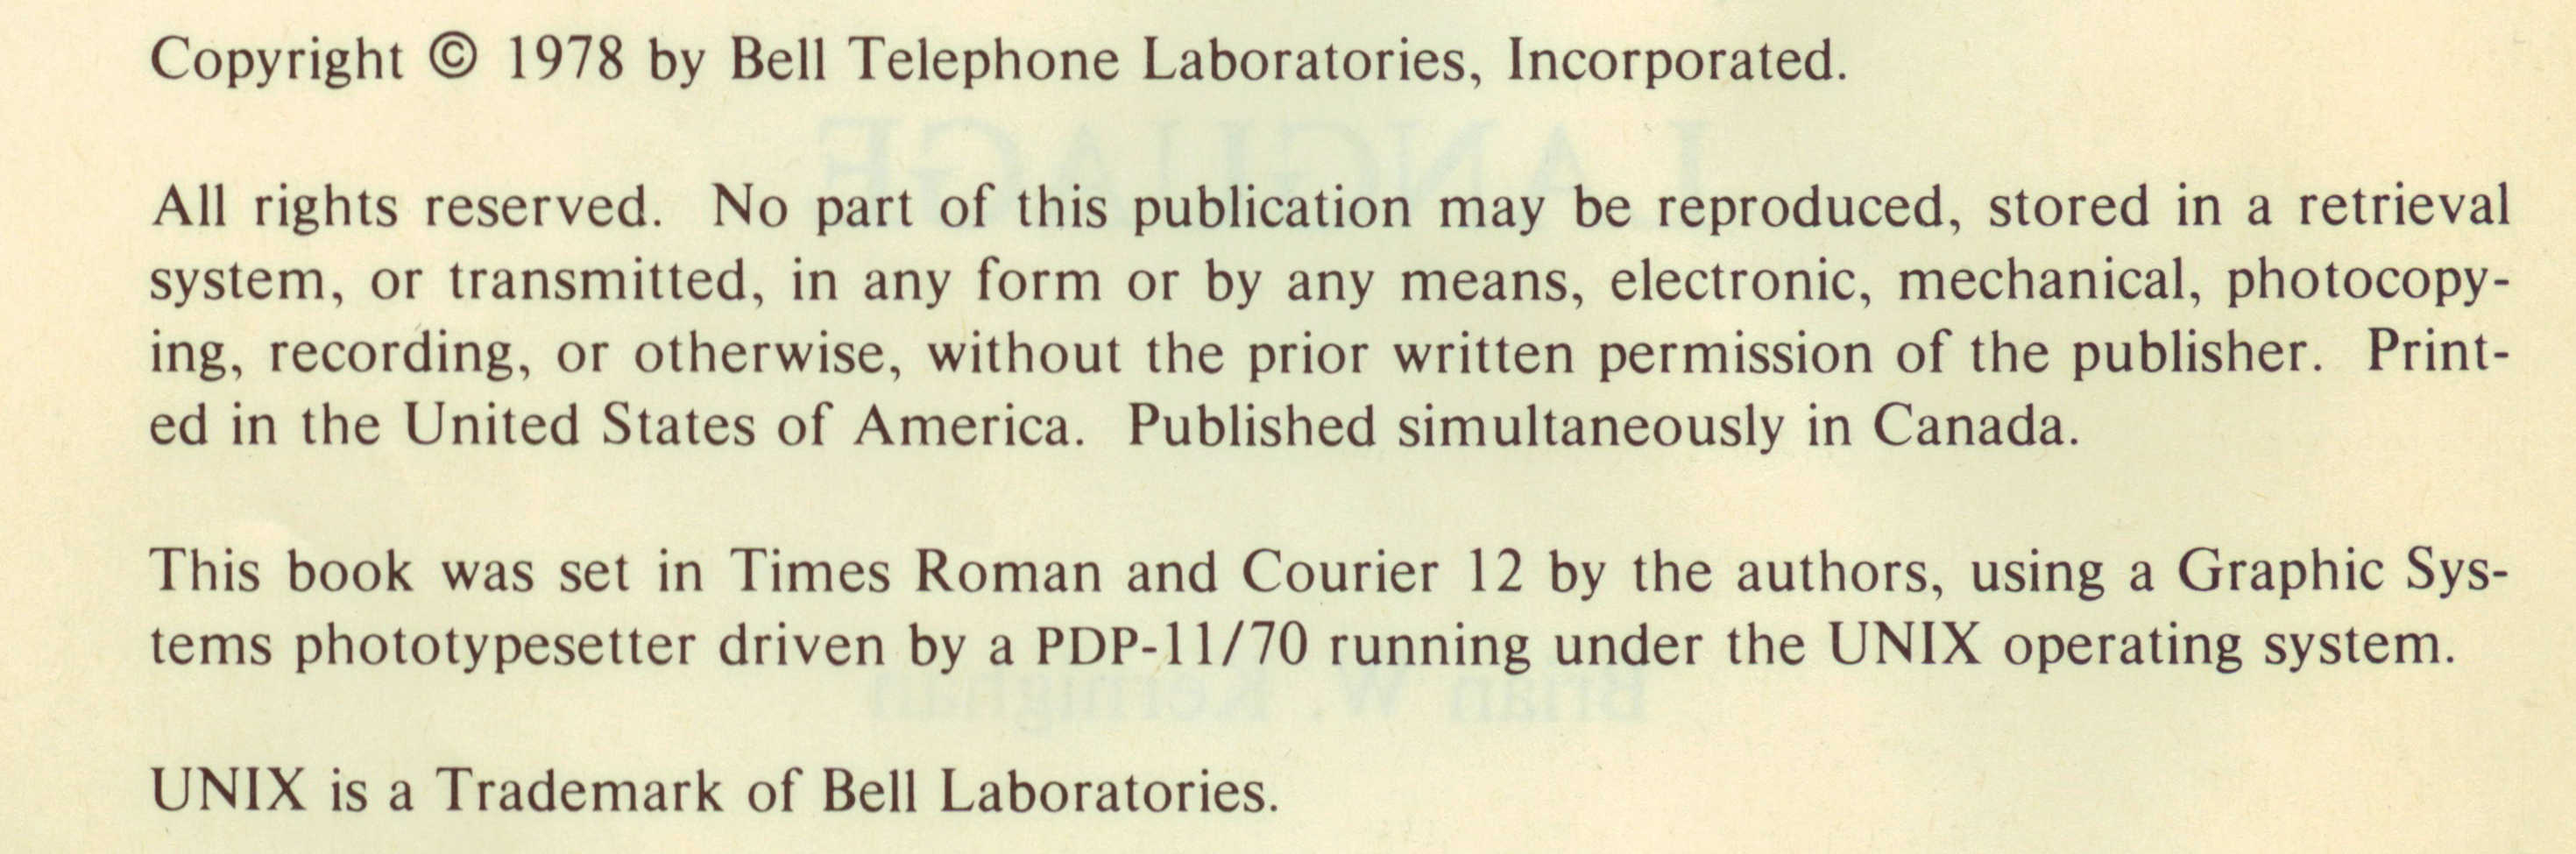
\includegraphics[width=11cm]{copyright.jpg} 
\end{frame}

\begin{frame}{The Big Picture}{Die Herstellung}
 \begin{block}{Gegeben}
  \vspace{-3mm}
  \begin{itemize}
   \item eine Hardware
   \item korrekte\footnote{meistens} Sourcefiles 
   \begin{itemize}
    \item haupts�chlich \C
    \item verstreut auf der Welt
    \item selber geschrieben
   \end{itemize}
  \end{itemize}
 \end{block}
 \vspace{-5mm}
 \begin{block}{Gesucht}
  \vspace{-3mm}
  \begin{itemize}
   \item ein Produkt
   \begin{itemize}
    \item z.B. ein \linux basiertes eingebettetes System
   \end{itemize}
  \end{itemize}
 \end{block}
 \vspace{-5mm}
 \begin{block}{L�sungsweg}
  \vspace{-3mm}
  \begin{itemize}
   \item z.B. \yocto
   \item oder etwas anderes
  \end{itemize}
 \end{block}
\end{frame}

\begin{frame}{Das Problem}{die richtige Wahl}
 \begin{itemize}
  \item die {\Huge richtigen} Sourcefiles
  \item {\Huge richtig} konfiguriert
 \end{itemize}
\end{frame}
